\providecommand{\main}{../../..}
\documentclass[\main/main.tex]{subfiles}
\begin{document}

\subsection{Esercizio 1}

Si definisca brevemente il concetto di impatto in un problema decisionale complesso, specificando che ruolo svolga nel processo decisionale.

Si descrivano alcune possibili rappresentazioni degli impatti di un problema finito (cioè con un numero finito, e piuttosto piccolo, di alternative).

Che cosa si intende dicendo che due impatti sono indifferenti? E incomparabili?

\subsection{Soluzione esercizio 1}
Gli impatti descrivono tutto ciò che è rilevante ai fine della decisione. Essi vengono modellati matematicamente tramite la \textbf{funzione impatto} $f: X \times \Omega \rightarrow F$, dove $F$ è l'insieme degli impatti possibili, $\Omega$ quello degli esiti possibili ed $X$ quello delle decisioni possibili.

Le componenti $f_l$ di una funzione impatto $f$ vengono chiamate \textbf{indicatori} e definiscono un aspetto dell'impatto.

Nel caso \textbf{finito} gli impatti possono essere rappresentati tramite la \textbf{matrice di valutazione}, le cui righe sono le \textit{configurazioni} $(x,\omega)$ mentre le colonne sono gli \textit{indicatori} $f_l$ ed in ogni cella vi è il valore dell'indicatore per quella configurazione.

In alternativa è possibile utilizzare la \textbf{rosa dei venti} (\ref{rosa_dei_venti}), un grafico bidimensionale:

\begin{figure}
  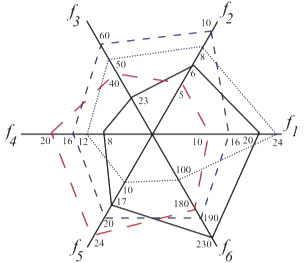
\includegraphics[width=0.5\textwidth]{rosa}
  \caption{Rosa dei venti}
  \label{rosa_dei_venti}
\end{figure}

Due impatti sono \textbf{indifferenti} quando il decisore accetta di scambiarli in entrambi i versi: $f_1 \preceq f_2  \land f_2 \preceq f_1 \Rightarrow f_1 \approx f_2$.

Due impatti sono \textbf{incomparabili} quando il decisore non accetta di scambiarli in alcun verso: $f_1 \npreceq f_2  \land f_2 \npreceq f_1 \Rightarrow f_1 \bowtie f_2$.

\end{document}